%% WEEK 1

\chapter{Graphs and Colourings} \label{Ch2:CH}
\thispagestyle{empty}

Much of this course will be about graphs, and a surprising amount of what we want to know about a graph can be phrased as a question about colouring it. We begin with the vocabulary, and then settle the first such question completely: which graphs admit a colouring with only two colours. We then ask the same question of hypergraphs, where it becomes considerably harder---even pinning down how many edges a $3$-uniform hypergraph needs before two colours are no longer enough takes real work. We then colour graphs with as many colours as it takes, and find that the number needed can be forced up as far as we like without ever creating a short cycle. Last, we colour the plane itself, an infinite graph whose chromatic number we can only trap between $4$ and $7$. The hypergraphs get a chapter of their own after that, and the opposite question---how large a complete graph must be before every colouring of its edges is forced to produce something monochromatic---gets one too, \Cref{Ch6:CH}.

\begin{boxnotation} \hfill
    \begin{itemize}
        \item $[k]$ will denote $\set{1, \ldots, k}$.
        \item $\sim$ will denote the adjacency relation on graph vertices.
        \item $K_n$ will denote the complete graph on $n$ vertices.
        \item $\H$ will denote the set of hyper-edges of a hypergraph $H$, and likewise for any other letter; calligraphic letters will denote families of sets more generally.
    \end{itemize}
\end{boxnotation}

\section{Colourings}

\begin{boxdefinition}[Colouring]
    Given a graph $G = (V, E)$, a $k$-colouring of $G$ is a map $c : V \to [k]$ such that $u \sim v \implies c(u) \ne c(v)$.
\end{boxdefinition}

\subsection{$2$-Colourings of Graphs}

Let's start with a motivating question: which graphs can be 2-coloured?

Any odd cycle graph can't be 2-coloured. That is, any graph that looks like
\begin{figure}[H]
    \centering
    \begin{tikzpicture}
        \cyclegraph{3}
        \begin{scope}[xshift = 3cm]
            \cyclegraph{5}
        \end{scope}
        \begin{scope}[xshift = 6cm]
            \cyclegraph{7}
        \end{scope}
        \node at (8.25, 0.1) {$\cdots$};
    \end{tikzpicture}
\end{figure}

Let's study when odd cycles exist.

\begin{boxlemma}\label{Ch2:Lemma:Odd_Closed_Walk}
    If $G$ has an odd closed walk, then $G$ has an odd cycle.
\end{boxlemma}
Recall that a closed walk need not be a cycle: walks can contain repetitions. So even line graphs can have closed walks (start from one vertex, go to its neighbour, return).
% [CORRECTED] was: "there must be some $x_i, x_j$ such that $x_i = x_j$ even though $i \neq j$" --- every closed walk
% has $x_1 = x_{\ell}$, so that says nothing, and at $i = 1$, $j = \ell$ the two sub-walks below are the length-$0$ walk
% and $W$ itself, neither shorter, so the minimality contradiction never fires.
\begin{proof}
    Suppose $G$ has an odd closed walk. Let $W$ be such a walk of minimal length. Write $W = \parenth{x_1, \ldots, x_i, \ldots, x_j, \ldots, x_{\ell}}$, with $x_{\ell} = x_1$. Suppose $W$ is not a cycle. Then there must be some $x_i, x_j$ such that $x_i = x_j$ with $1 \leq i < j \leq \ell - 1$, ie, there must be some repetition beyond the closing one. Then, $\parenth{x_1, \ldots, x_i, x_{j+1}, \ldots, x_{\ell}}$ and $\parenth{x_i, x_{i+1}, \ldots, x_{j}}$ are both shorter walks than $W$. Moreover, one of them must be of odd length. This contradicts minimality of the length of $W$. So $W$ must be a cycle.
\end{proof}

Here's a cool result.

\begin{boxtheorem}
    A graph $G = (V, E)$ can be $2$-coloured if and only if $G$ has no odd cycle.
\end{boxtheorem}
\begin{iffproof}
    \onlyifdir We've already seen that odd cycles can't be $2$-coloured. So if $G$ can be $2$-coloured, it can't have an odd cycle. We've essentially seen this from the examples above.

    \ifdir We may assume $G$ is connected, since otherwise we can colour each component separately. Fix some $v_0 \in V$. Define $c : V \to \set{1, 2}$ by
    \begin{align*}
        c(u) =
        \begin{cases}
            2 & \text{ if } \dist{v_0, u} \text{ is odd} \\
            1 & \text{ if } \dist{v_0, u} \text{ is even}
        \end{cases}
    \end{align*}
    where $\dist{\cdot, \cdot}$ denotes the shortest number of edges from one vertex to another.

    We claim that this $c$ is a valid $2$-colouring.

    Indeed, suppose it is not. Then, there must be some $u, v \in V$ such that $u \sim v$ and $c(u) = c(v)$. Now let's consider the two possible cases on the colour.

    Suppose $c(u) = c(v) = 1$ for adjacent $u, v$. Then, there is a path of even length between $v$ and $v_0$ and another path of even length between $u$ and $v_0$. Concatenating the path from $v$ to $v_0$ with the one from $v_0$ to $u$, and closing up with the edge $uv$, we get a closed walk of length even $+$ even $+ 1$. This is odd, so by \Cref{Ch2:Lemma:Odd_Closed_Walk}, $G$ has an odd cycle.

    The case $c(u) = c(v) = 2$ is identical: the two paths are now of odd length, so the closed walk they form with the edge $uv$ has length odd $+$ odd $+ 1$, which is odd again.

    Either way, $G$ has an odd cycle, contrary to hypothesis. So $c$ must be a valid $2$-colouring.
\end{iffproof}

\subsection{Colourings of Hypergraphs}

Colouring is not really a question about graphs. All the definition above asks of $G$ is that we know which pairs of vertices may not share a colour, and nothing stops us forbidding larger sets instead.

\begin{boxdefinition}[Hypergraph] \label{Ch2:Def:Hypergraph}
    Given a vertex set $V$, a \textbf{hypergraph} is a pair $H = \parenth{V, \H}$, where $\H$ is a collection of subsets of $V$. The sets in $\H$ are called \textbf{hyper-edges}.
\end{boxdefinition}

\begin{boxdefinition}[Uniformity]
    A hypergraph $H$ is \textbf{$k$-uniform} if $\abs{f} = k$ for all $f \in \H$.
\end{boxdefinition}

The following is thus obvious.

\begin{boxproposition}
    A graph is a $2$-uniform hypergraph.
\end{boxproposition}

\begin{boxdefinition}
A proper colouring of a hypergraph $H$ is an assignment $c : V \to [r]$ such that $\forall f \in \H$, $\abs{c(f)} \geq 2$.
\end{boxdefinition}

We say ``no edge is monochromatic''.

We can ask ourselves the following question: \textbf{``Which $3$-uniform hypergraphs are $2$-colourable?}

For each $k$, define $m(k)$ to be the smallest $m$ such that $\exists$ some $k$-uniform hypergraph with $m$ edges that is not $2$-colourable. We can show that $m(2) = 3$. But what is $m(3)$? That is, how many $3$-edges do I need to prevent $2$-colourability?

\subsection{The Value of $m(3)$}

Let $H$ be a $3$-uniform hypergraph that's not $2$-colourable. Assume, further, that $H$ has at most $6$ edges (each being a subset of size $3$).

First, we'll show that we can reduce, without loss of generality, to the case where $H$ has exactly $6$ vertices. Indeed, if $H$ has vertices $x, y$ that are not in any common edge, then I can define $H'$ by ``merging'' $x$ and $y$. So $H'$ has one fewer vertex than $H$. This $H'$ cannot be $2$-colourable: if it were, then that colouring would extend to $H$ by using the colour of the merged vertex at both $x$ and $y$, which would make $H$ $2$-colourable. And when $H$ has more than $6$ vertices, such a pair always exists.

An edge has $3$ vertices, so it covers the $\binom{3}{2} = 3$ pairs among them, and $H$ has at most $6$ edges, so at most
\begin{align*}
    6 \cdot \binom{3}{2} = 18
\end{align*}
pairs are covered in total. But if $H$ has $n \geq 7$ vertices, there are $\binom{n}{2} \geq \binom{7}{2} = 21$ pairs to cover. So some pair is left uncovered, and merging it brings us one vertex closer to $6$.

So now assume that $H$ has exactly $6$ edges and $6$ vertices and is not $2$-colourable.

There is no loss in the vertex count in the other direction either: a hypergraph with fewer than $6$ vertices can be handed as many extra vertices as it likes, and vertices lying in no edge change nothing about which colourings are proper.

Now count colourings. Among all the ways of colouring $6$ vertices with two colours, consider only the balanced ones, which split $V$ into two sets of three; there are $\frac{1}{2}\binom{6}{3} = 10$ of these. Such a colouring fails exactly when some edge is monochromatic, and an edge of $H$ has three vertices, so it is monochromatic under a balanced colouring precisely when it is one of the two colour classes. Each edge $f$ therefore rules out exactly one of the ten balanced colourings, namely the one splitting $V$ into $f$ and $V \setminus f$. Six edges rule out at most six of the ten, so at least four survive, and any one of them is a proper $2$-colouring of $H$. This contradicts our assumption, so no such $H$ exists and
\begin{align*}
    m(3) \geq 7
\end{align*}

% Not from the lecture: the example and proposition below were supplied to close the
% m(3) question the reduction above sets up.
That bound is attained, and the hypergraph attaining it is a familiar object.

\begin{boxexample}[The Fano Plane]
    The \textbf{Fano plane} is the $3$-uniform hypergraph on the seven vertices below, whose seven edges---by convention, its \textbf{lines}---are the three sides of the triangle, the three medians, and the circle through the three edge midpoints.
\end{boxexample}

\begin{figure}[H]
    \centering
    \begin{tikzpicture}
        \fanoplane
    \end{tikzpicture}
\end{figure}

Every vertex lies on exactly three lines, any two vertices lie on exactly one line together, and any two lines meet in exactly one vertex. That last property is what does the work below.

\begin{boxproposition}
    The Fano plane is not $2$-colourable. Hence $m(3) = 7$.
\end{boxproposition}
\begin{proof}
    Of the $\binom{7}{4} = 35$ sets of four vertices, exactly $28$ contain a line: a line together with any one of the four vertices off it gives such a set, which is $7 \cdot 4 = 28$ sets in all, and no two of them coincide because four vertices cannot contain two lines---two lines meet in a vertex, so between them they cover five. The seven sets left over are the complements of the seven lines.

    Now suppose we had a proper $2$-colouring, with colour classes $A$ and $B$, and say $\abs{A} \leq 3$. If $\abs{A} = 3$, then $A$ is not a line, since $A$ is monochromatic; so $B = V \setminus A$ is a set of four vertices that is not the complement of a line, and hence contains one. If $\abs{A} \leq 2$, then the vertices outside $B$ lie on at most $3 + 3 - 1 = 5$ lines between them, so at least two lines avoid them both and lie inside $B$. Either way some line is monochromatic, which is a contradiction.

    So the Fano plane is a $3$-uniform hypergraph with seven edges that is not $2$-colourable, giving $m(3) \leq 7$.
\end{proof}

\subsection{Bounds on $m(k)$}

Pinning down $m(3)$ took a page of case analysis, and doing the same for $m(4)$ is out of the question. What we can do for every $k$ at once is bound it, and the lower bound falls out of an idea that will keep coming back: colour at random, and show that a bad colouring is improbable.

\begin{boxtheorem}\label{Ch2:Thm:mk_Lower_Bound}
    $m(k) \geq 2^{k - 1}$. In other words, any $k$-uniform hypergraph with $< 2^{k - 1}$ edges is $2$-colourable.
\end{boxtheorem}
\begin{proof}
    Given a hypergraph with $< 2^{k-1}$ edges, randomly colour the vertices red and blue, with equal probability ($1/2$) for each. For each edge $f$, let $\mathcal{E}_f$ be the event that $f$ is monochromatic. Then,
    \begin{align*}
        \Pr\of{\mathcal{E}_f} = \frac{2}{2^k}
    \end{align*}
    Taking a simple union bound,
    \begin{align*}
        \Pr\of{\bigcup_{f \in \H} \mathcal{E}_f} \leq \frac{\abs{\H}}{2^{k - 1}} < 1
    \end{align*}
    where we interpret $\bigcup_{f \in \H} \mathcal{E}_f$ as the event that there is a monochromatic edge. As the probability is less than $1$, there must be at least one colouring with no monochromatic edge.
\end{proof}

Note that the above argument can also be written combinatorially instead of probabilistically. In this instance, the probabilistic language essentially conveys the same information as combinatorial language would. But this may not always be true, so it's worth being careful about this.

In the other direction, the truth is only a factor of about $k^2$ away.

\begin{boxexercise}
    Prove that $m(k) = \BigO{k^2 \cdot 2^k}$
\end{boxexercise}

\subsection{Maker-Breaker Games}

% [CORRECTED] was: "that one of two players be able to build such a colouring one vertex at a time, against an opponent
% trying to stop them" --- a breaker win only keeps maker's class free of an edge; breaker's own class may contain one,
% so the play does not build a proper $2$-colouring. "Far more demanding" does stand: breaker winning implies
% $2$-colourability, by setting breaker's second-player strategy against the first-player one it yields.
\Cref{Ch2:Thm:mk_Lower_Bound} says that a hypergraph with few enough edges has a proper $2$-colouring somewhere among all the colourings of its vertices. It turns out that the very same threshold survives a far more demanding requirement: that one of two players, claiming vertices one at a time, be able to stop the other from ever owning a whole edge. Winning that does not by itself produce a proper $2$-colouring, since the winner's own class may contain a monochromatic edge. It does force one to exist all the same: a breaker who can win going second can also win going first, by holding a spare vertex in reserve, and setting those two strategies against each other leaves neither class containing an edge.

Here's a fun fact: a ``maker-breaker'' game is a game where the ``maker'' wins if they are able to achieve an objective and the ``breaker'' wins if they are able to stop the maker from winning. So if you set up a ``maker-breaker'' version of tic-tac-toe, where only the crosses can win by making three in a row and the noughts can only win by stopping the crosses, the crosses will always win (assuming the crosses play first). This is, of course, different from tic-tac-toe, which, as our own studies from when we were a kid have shown, can always be drawn.

% [CORRECTED] was: "the game is $2$-colouring; maker winning is equivalent to the existence of a colouring with a
% monochromatic edge; and breaker winning is equivalent to the inexistence of such edge" --- colouring everything red
% makes an edge monochromatic in every hypergraph with a nonempty edge, so that condition holds always and can be
% equivalent to nothing. Winning is a property of strategies, not of which colourings exist.
In the language of hypergraphs, the game is played on the vertices of $H$: the two players alternately claim unclaimed vertices, maker wins by claiming every vertex of some edge, and breaker wins if play ends with no edge wholly maker's.

Whether breaker can hold out depends not only on how many edges there are, but on how many of them pass through a single vertex.

\begin{boxlemma} \label{Ch2:Lemma:Maker_Breaker_Degree}
    Let $H$ be a $k$-uniform hypergraph with $m$ edges and maximum degree
    \begin{align*}
        \Delta = \max_{v \in V} \abs{\setst{f \in \H}{v \in f}}
    \end{align*}
    If $m + \Delta < 2^k$, then breaker wins (if breaker goes second).
\end{boxlemma}
\begin{proof}
    At the start of move $i$, we will conceptualise the danger of edge $f \in \H$ by
    \begin{align*}
        \phi_i(f) &=
        \begin{cases}
            2^{\text{number of maker moves in $f$}} & \text{ if there are no breaker moves in $f$} \\
            0 & \text{ if there is a breaker move in $f$} \\
        \end{cases}
        \\
        \Phi_i &= \sum_{f \in \H} \phi_i(f)
    \end{align*}
    Consider the strategy where, once maker has played $y$ on move $i$, breaker plays the unclaimed vertex carrying the most danger, that is, the $x$ maximising
    \begin{align*}
        \sum_{f \ni x} \phi(f)
    \end{align*}
    with $\phi$ measured after maker's move. Two things move $\Phi$ on move $i$. Maker's play doubles the danger of every edge through $y$ that breaker has not already killed, so it raises $\Phi$ by $a_i = \sum_{f \ni y} \phi_i(f)$; breaker's play sends the danger of every surviving edge through $x$ to $0$, so it lowers $\Phi$ by the quantity $b_i$ that breaker has just maximised. Hence
    \begin{align*}
        \Phi_{i + 1} = \Phi_i + a_i - b_i
    \end{align*}

    The point of breaker's rule is that $a_i \leq b_{i - 1}$ for every $i \geq 2$. Indeed, $y$ is unclaimed right up until maker takes it on move $i$, so it was one of the vertices breaker was choosing between on move $i - 1$, and breaker chose one carrying at least as much danger as it. Between then and the start of move $i$ nothing happens except breaker's own play, which only ever sends dangers to $0$, so the danger through $y$ at the start of move $i$ is no greater than it was when breaker passed $y$ over.

    Summing $\Phi_{i + 1} = \Phi_i + a_i - b_i$ over the first $n$ moves and cancelling each $a_i$ against $b_{i - 1}$, everything past the first two terms disappears and we are left with
    \begin{align*}
        \Phi_{n + 1} \leq \Phi_1 + a_1
    \end{align*}
    Stopping the same sum one term earlier gives the same bound halfway through a move, after maker has played and before breaker has replied. Now $\Phi_1 = m$, since at the start every edge contains a move of neither player and so contributes $2^0 = 1$, and $a_1$ is the number of edges through maker's opening vertex, which is at most $\Delta$. So the danger never exceeds $m + \Delta$ at any point in the game.

    But if maker ever completes an edge $f$, then at that moment $f$ contains all $k$ of its vertices from maker and none from breaker, so $\phi(f) = 2^k$ and hence $\Phi \geq 2^k$. Since $m + \Delta < 2^k$, this never happens, and breaker wins.
\end{proof}

No vertex lies in more edges than there are, so $\Delta \leq m$, and the threshold at which breaker can hold out is exactly the one we have just been looking at.

\begin{boxcorollary}[\Erdos-Selfridge]
    If $H$ is a $k$-uniform hypergraph with $m$ edges, and $m < 2^{k - 1}$, then breaker wins (if breaker goes second).
\end{boxcorollary}
\begin{proof}
    $m + \Delta \leq 2m < 2^k$, so \Cref{Ch2:Lemma:Maker_Breaker_Degree} applies.
\end{proof}

Let's consider higher-dimensional maker-breaker tic-tac-toe.

\begin{boxexample}
    Turns out that $8 \times 8 \times 8$ maker-breaker tic-tac-toe is breaker-winnable: we can show that $m = \frac{10^3 - 8^3}{2} = 244$ and $\Delta = 7$, meaning $m + \Delta = 251 < 2^k = 256$.
\end{boxexample}

% [CORRECTED] was: "the lines are in bijection with the pairs of shell cells, of which there are
% $\frac{10^3 - 8^3}{2}$" --- the shell has $488$ cells and so $\binom{488}{2} = 118{,}828$ pairs; $244$ counts the
% pairs that are the two ends of a line, which is a perfect matching on the shell rather than all of its pairs.
Both numbers come out of the geometry. For $m$, pad the board with one extra cell in every direction, giving a $10 \times 10 \times 10$ cube, and run each winning line one step past each of its two ends. The two cells we land on lie in the shell we just added, and every cell of the shell is the end of exactly one line: a coordinate of the cell equal to $0$ tells the line to increase along that axis, one equal to $9$ tells it to decrease, and the rest stay fixed. So the lines are in bijection with those pairs of shell cells that arise as the two ends of a line, and since every shell cell is the end of exactly one line there are $\frac{10^3 - 8^3}{2}$ of them. For $\Delta$, a line through a given cell is determined by its direction, and a corner cell has the $3$ lines along the axes, the $3$ face diagonals and the one long diagonal through it, which is $7$; no cell of an $8 \times 8 \times 8$ board does better. And it is \Cref{Ch2:Lemma:Maker_Breaker_Degree} doing the work here rather than the corollary, since $244$ is a long way above $2^{k - 1} = 128$.

We won't say any more about tic-tac-toe in this course, but it was a fun aside.

\section{Chromatic Number}

Back to colouring vertices, and this time we are not rationed to two colours. \Cref{Ch2:CH} opened by asking which graphs can be coloured with two of them; the question now is how many colours a graph needs in general, and how far that number can be pushed away from the obvious lower bound.

\begin{boxdefinition}[Chromatic Number] \label{Ch2:Def:Chromatic_Number}
    The \textbf{chromatic number} of a graph $G$, denoted $\chi(G)$, is the smallest number of colours I need to colour $G$.
\end{boxdefinition}

\subsection{Trivial Bounds}

There are some trivial bounds on $\chi(G)$.

% [CORRECTED] was: "a fully connected subgraph" --- "connected" already means path-connected in these notes (the proof
% of the $2$-colouring theorem in 1.1.1 colours each component separately), and on that reading every path would be a clique in itself, so $\omega(P_n) = n$
% while $\chi(P_n) = 2$ and the inequality below fails. What $\omega \leq \chi$ needs is pairwise adjacency.
\begin{boxdefinition}[Clique]
    A \textbf{clique} in $G$ is a complete subgraph, ie, a set of vertices any two of which are adjacent. The \textbf{clique number} of a graph, denoted $\omega(G)$, is the number of vertices in the largest clique.
\end{boxdefinition}

It isn't hard to see that $\omega(G) \leq \chi(G)$ always. Similarly, it is clear that $\chi(G) \leq \Delta + 1$, where $\Delta$ is the maximum degree.

The upper-bound is absolutely not tight, for instance we can have a ``star graph'' with one vertex in the middle connected to a number of other vertices. This has high $\Delta$ but $\chi(G) = 2$.

\begin{figure}[H]
    \centering
    \begin{tikzpicture}
        \colouredstargraph[1.15]{8}{red}{blue}
    \end{tikzpicture}
\end{figure}

Similarly, the lower-bound is also not tight. For example, any odd cycle on more than $3$ vertices (eg, the $5$-cycle) has clique number $2$ but chromatic number $3$.

\begin{figure}[H]
    \centering
    \begin{tikzpicture}
        \colouredcyclegraph[1.15]{5}{red, blue, red, blue, green!60!black}
    \end{tikzpicture}
\end{figure}

In fact, we will show that $\chi(G)$ can be much bigger than $\omega(G)$.

\subsection{Perfect Graphs}

First, the graphs for which the lower bound is exact---and stays exact when we throw vertices away. That needs a word for what is left when we do.

% [FILLED] the lecture used the term without defining it; the definition below was supplied
\begin{boxdefinition}[Induced Subgraph]
    Given a graph $G = \parenth{V, E}$ and a subset $W \ssq V$, the subgraph of $G$ \textbf{induced} by $W$, denoted $G[W]$, is the graph with vertex set $W$ whose edges are precisely the edges of $G$ with both endpoints in $W$. An \textbf{induced subgraph} of $G$ is any subgraph of the form $G[W]$.
\end{boxdefinition}

\begin{boxdefinition}[Perfect Graph]
    A graph $G$ is \textbf{perfect} if $\chi(H) = \omega(H)$ for all induced subgraphs $H$ of $G$.
\end{boxdefinition}

\subsection{Zykov's Construction}

At the opposite extreme are graphs with $\omega = 2$ and $\chi$ as large as we like, and we can build them by hand.

Let's now construct a sequence $(G_n)_{n \in \N}$. Start with $G_1$ a single vertex. Given $G_1, \ldots, G_{k-1}$, take disjoint copies of all of them, and for every way of choosing one vertex $v_i$ from each $G_i$ add a new vertex adjacent to $v_1, \ldots, v_{k-1}$ and to nothing else; the result is $G_k$. There are $\abs{G_1} \cdots \abs{G_{k-1}}$ new vertices, so $G_2$ has $1 + 1 = 2$ vertices and is a single edge, $G_3$ has $1 + 2 + 2 = 5$ and is the $5$-cycle, and $G_4$ has $1 + 2 + 5 + 10 = 18$ (the construction is due to Zykov).

\begin{figure}[H]
    \centering
    \begin{tikzpicture}
        \node[circle, fill = black, inner sep = 1.5pt] (a1) at (0, 0) {};
        \node[anchor = north] at (0, -0.5) {$G_1$};
        \begin{scope}[xshift = 1.75cm]
            \node[circle, fill = black, inner sep = 1.5pt] (a2) at (0, 0) {};
            \node[circle, fill = black, inner sep = 1.5pt] (b2) at (1, 0) {};
            \draw (a2) -- (b2);
            \node[anchor = north] at (0.5, -0.5) {$G_2$};
        \end{scope}
        \begin{scope}[xshift = 4.5cm]
            \foreach \v [count = \i from 0] in {a3, d3, b3, c3, e3}{
                \node[circle, fill = black, inner sep = 1.5pt] (\v) at (\i, 0) {};
            }
            \draw (a3) -- (d3) -- (b3) -- (c3) -- (e3);
            \draw (a3) to[bend left = 40] (e3);
            \node[anchor = north] at (2, -0.5) {$G_3$};
        \end{scope}
    \end{tikzpicture}
\end{figure}

$G_4$ is already hard to take in, but the shape of the construction survives in it: the three earlier graphs across the top, and below them one new vertex for each of the $1 \cdot 2 \cdot 5 = 10$ ways of picking one vertex from each. The edges into the copies are drawn faintly, so that the copies themselves stay visible.

\begin{figure}[H]
    \centering
    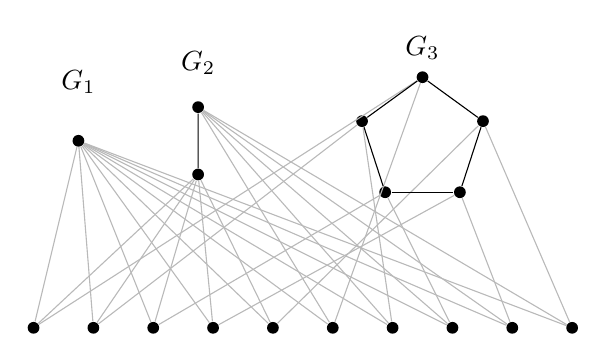
\begin{tikzpicture}[scale = 0.95]
        \node[circle, fill = black, inner sep = 1.5pt] (u) at (0, 1) {};
        \node[anchor = south] at (0, 1.5) {$G_1$};
        \node[circle, fill = black, inner sep = 1.5pt] (v1) at (1.6, 0.55) {};
        \node[circle, fill = black, inner sep = 1.5pt] (v2) at (1.6, 1.45) {};
        \node[anchor = south] at (1.6, 1.75) {$G_2$};
        \foreach \k in {1, ..., 5}{
            \pgfmathsetmacro{\ang}{90 + 72 * (\k - 1)}
            \pgfmathsetmacro{\wx}{4.6 + 0.85 * cos(\ang)}
            \pgfmathsetmacro{\wy}{1 + 0.85 * sin(\ang)}
            \node[circle, fill = black, inner sep = 1.5pt] (w\k) at (\wx, \wy) {};
        }
        \node[anchor = south] at (4.6, 1.95) {$G_3$};
        \foreach \j in {1, 2}{
            \foreach \k in {1, ..., 5}{
                \pgfmathtruncatemacro{\i}{5 * (\j - 1) + \k}
                \pgfmathsetmacro{\x}{-0.6 + 0.8 * (\i - 1)}
                \node[circle, fill = black, inner sep = 1.5pt] (x\i) at (\x, -1.5) {};
                \draw[gray!55, thin] (x\i) -- (u);
                \draw[gray!55, thin] (x\i) -- (v\j);
                \draw[gray!55, thin] (x\i) -- (w\k);
            }
        }
        \draw (v1) -- (v2);
        \foreach \k in {1, ..., 5}{
            \pgfmathtruncatemacro{\next}{mod(\k, 5) + 1}
            \draw (w\k) -- (w\next);
        }
    \end{tikzpicture}
\end{figure}

These have exactly the property we want.

\begin{boxproposition} \label{Ch2:Prop:Zykov}
    For every $k \geq 1$, $G_k$ has no triangles and $\chi(G_k) = k$.
\end{boxproposition}
\begin{proof}
    Both by induction on $k$, and both trivial for $G_1$. The new vertices of $G_k$ form an independent set, and the neighbours of any one of them lie one in each of $G_1, \ldots, G_{k-1}$, so no two of them are adjacent. A triangle can therefore contain at most one new vertex, and if it contains one then its other two vertices are adjacent neighbours of that vertex, which do not exist. So every triangle of $G_k$ lies inside some $G_i$, and by induction there are none.

    For $\chi(G_k) \leq k$, colour each $G_i$ with $i \leq k - 1$ colours, which we can by induction, and give every new vertex colour $k$. For $\chi(G_k) \geq k$, suppose $c$ is a proper $(k-1)$-colouring of $G_k$. Its restriction to $G_i$ is a proper colouring of $G_i$, and so uses at least $\chi(G_i) = i$ colours. Pick $v_1 \in G_1$; $G_2$ uses at least two colours, so pick $v_2 \in G_2$ with $c(v_2) \neq c(v_1)$; $G_3$ uses at least three, so pick $v_3 \in G_3$ with $c(v_3) \notin \set{c(v_1), c(v_2)}$; and so on, at each step choosing $v_i \in G_i$ to avoid the $i - 1$ colours chosen so far. After $k - 1$ steps, $c(v_1), \ldots, c(v_{k-1})$ are $k - 1$ distinct colours, which is all of them, and the new vertex attached to $v_1, \ldots, v_{k-1}$ has no colour left.
\end{proof}

\subsection{Graphs of Large Girth}

The graphs of \Cref{Ch2:Prop:Zykov} have no triangles, but nothing stops them having cycles of length four or five---$G_3$ is one. It is natural to ask whether forbidding all short cycles finally holds the chromatic number down, and the answer is that it does not.

\begin{boxdefinition}[Girth]
    The \textbf{girth} of $G$, denoted $\girth(G)$, is the length of the shortest cycle in $G$.
\end{boxdefinition}

% [CORRECTED] was: "The girth of a cycle is infinite." --- the girth of $C_n$ is $n$; it is a graph with no cycles at
% all whose girth the definition leaves open, and $\infty$ is the standard value there.
The girth of a graph with no cycles is infinite.

% [CORRECTED] was: "graphs of girth $k$ and chromatic number $k$" --- the argument below produces a graph with no cycle
% of length $\leq k$, so its girth is not $k$ but greater, and it bounds the chromatic number below without pinning it
% down; and no simple graph has girth $1$ or $2$. The exact version does follow for $k \geq 3$ (delete vertices until
% $\chi = k$, then add a disjoint $C_k$), but that is not what is proved here.
\begin{boxtheorem}[\Erdos] \label{Ch2:Thm:Erdos_Girth}
    For any $k$, there are graphs of girth at least $k$ and chromatic number at least $k$.
\end{boxtheorem}

The proof runs through independent sets rather than through colourings directly.

\begin{boxdefinition}[Independence Number]
    A set $S$ of vertices of $G$ is \textbf{independent} if no two of its elements are adjacent. The \textbf{independence number} of $G$, denoted $\alpha(G)$, is the size of the largest independent set in $G$.
\end{boxdefinition}

We know we can construct graphs of average degree $d$ with $\frac{nd}{2}$ edges. We want to prove that such a graph has a ``large'' independent set.

As a first attempt, let's choose a set $S$ randomly by including each vertex of $G$ independently with probability $p$. Write $e(S)$ for the number of edges of $G$ with both endpoints in $S$, so that $S$ is independent exactly when $e(S) = 0$. Then,
\begin{align*}
    \E\of{\abs{S}} &= pn \\
    \E\of{e(S)} &= \frac{p^2 n d}{2}
\end{align*}
% [CORRECTED] was: "$\E\of{e(S)} \approx \sqrt{n / d}$" at the end of this paragraph --- at $p = \sqrt{2 / dn}$ the
% expected number of edges inside $S$ is exactly $1$, by the choice of $p$; it is $\E\of{\abs{S}} = \sqrt{2n / d}$ that
% comes out at about $\sqrt{n / d}$, and it is a size that the next sentence compares against $n / (d + 1)$.
the second line because each of the $\frac{nd}{2}$ edges lands inside $S$ with probability $p^2$. We want $S$ large and $e(S)$ small, and the two pull against each other: the expected size grows like $p$ but the expected number of edges inside like $p^2$. So we take $p$ as large as we can while keeping the expected number of edges inside $S$ down to about one. I would want $p \simeq \sqrt{\frac{2}{dn}}$. In that case we would get something like $\E\of{\abs{S}} \approx \sqrt{\frac{n}{d}}$. This is a poor return: a disjoint union of copies of $K_{d + 1}$ has average degree $d$ and an independent set of size $\frac{n}{d + 1}$, and the trouble is that we have insisted on $S$ coming out independent all by itself.

Now, let's make another attempt. Still choose $S$ randomly, including each vertex with probability $p$.

Let $X = \abs{S}$ and $Y = e(S)$.

% [CORRECTED] was: "So if $S$ has $X - Y$ many vertices then edges form an of $G$ contains an independent set of size
% $X - Y$", and "$\E\of{X - Y} = \frac{nd}{2}$" --- the first has no reading that is both well-formed and does the work
% (with $X = \abs{S}$ its hypothesis forces $Y = 0$); the second is the value at $p = 1/d$ of $pn - p^2 nd / 2$, which
% is $n / d - n / 2d = n / 2d$, and $nd / 2$ exceeds $n \geq X - Y$ as soon as $d > 2$.
Now consider $\E\of{X - Y}$. This is $pn - \frac{p^2 n d}{2}$ by linearity of expectation. So if $S$ has $X$ vertices and $Y$ edges inside it, then $G$ contains an independent set of size at least $X - Y$, and using $p = \frac{1}{d}$ gives $\E\of{X - Y} = \frac{n}{2d}$.

% [FILLED] the argument broke off after computing $\E\of{X - Y}$; the conclusion below and the lemma recording it were supplied
This needs $d \geq 1$ for $p = \frac{1}{d}$ to be a probability at all, and then some $S$ has $X - Y \geq \E\of{X - Y} = \frac{n}{2d}$. Now alter that $S$: for each of the $Y$ edges lying inside it, throw out one of the two endpoints. At most $Y$ vertices go, and no edge of $G$ keeps both its endpoints, so what is left is an independent set of size at least $X - Y \geq \frac{n}{2d}$.

What we have shown is worth recording.

\begin{boxlemma}
    If $G$ is a graph with $n$ vertices and average degree $d \geq 1$, then $G$ has an independent set of size at least $\frac{n}{2d}$.
\end{boxlemma}

The above is called the \textbf{method of alterations}---constructing something randomly and then changing based on how it goes.

The proof of \Cref{Ch2:Thm:Erdos_Girth} plays the same trick, but with a random graph in place of a random set of vertices.

% Not from the lecture: the lecture used $G_{n, p}$ without defining it, and the definition below was supplied.
\begin{boxdefinition}[Random Graph] \label{Ch2:Def:Random_Graph}
    For $n \in \N$ and $p \in [0, 1]$, the \textbf{random graph} $G_{n, p}$ is the graph on the vertex set $[n]$ in which each of the $\binom{n}{2}$ possible edges is present independently with probability $p$.
\end{boxdefinition}

\begin{proof}[Proof of \Cref{Ch2:Thm:Erdos_Girth}]
    Fix $k \geq 3$; for $k \leq 2$ a single edge already does. Consider the graph $G_{n, p}$ for $p = \frac{n^{\varepsilon}}{n}$. For some small $\varepsilon > 0$ (in particular, $\varepsilon \ll \frac{1}{k}$), we see that
    % [FILLED] the display broke off after the union bound; the second line and the paragraph after it were supplied
    \begin{align*}
        \Pr\of{\alpha\of{G_{n, p}} \geq a} &\leq \binom{n}{a} \parenth{1 - p}^{\binom{a}{2}}  \\
        & \leq n^a e^{-p \binom{a}{2}} = \exp\of{a \parenth{\ln n - \frac{p \parenth{a - 1}}{2}}}
    \end{align*}
    using $\binom{n}{a} \leq n^a$ and $1 - p \leq e^{-p}$. Take $a = \ceil{\frac{n}{2k}}$, so that $a - 1 \geq \frac{n}{2k} - 1$ and hence $\frac{p \parenth{a - 1}}{2} \geq \frac{n^{\eps}}{4k} - \frac{1}{2}$. Any positive power of $n$ eventually beats $\ln n$, so the bracket is negative for $n$ large enough and the whole thing tends to $0$: that is, $\Pr\of{\alpha\of{G_{n, p}} \geq \frac{n}{2k}} \to 0$ as $n \to \infty$.

    Now, let $X$ be the number of short cycles. That is, cycles of length $\leq k$. Then,
    \begin{align*}
        \E(X) &= \sum_{\ell = 3}^{k} \frac{\binom{n}{\ell} \cdot \ell !}{2\ell} p^{\ell} \\
        &\leq \frac{1}{2} \sum_{\ell = 3}^{k} n^{\ell} p^{\ell} \\
        &\leq \parenth{k - 2} \frac{1}{2} n^k p^k \\
        &\leq \frac{k}{2} n^{\eps k}
    \end{align*}
    % [CORRECTED] was: "as $\eps \to 0$" after the display --- with $n$ and $k$ fixed and $\eps \to 0$ the bound tends to
    % $k / n$, not $0$; it is $n \to \infty$ with $\eps k < 1$ fixed that sends $k n^{\eps k - 1}$ to $0$, and that is the
    % limit "for sufficiently large $n$" in the next sentence uses.
    By Markov's inequality (\Cref{Ch1:Thm:Markov}),
    \begin{align*}
        \Pr\of{X \geq \frac{n}{2}} \leq \frac{\E(X)}{n / 2} \to 0
    \end{align*}
    as $n \to \infty$. So, there is some graph $G$ with $n$ vertices, for sufficiently large $n$, such that $X \leq \frac{n}{2}$ and $\alpha(G) \leq \frac{n}{2k}$. Construct a new graph $G'$ by deleting one vertex from each short cycle. This new graph has at least $\frac{n}{2}$ vertices, independence number at most $\frac{n}{2k}$, and thus chromatic number at least $\frac{n/2}{n/2k} \geq k$.
\end{proof}

\section{The Chromatic Number of the Plane}

Every graph so far has been finite. The plane gives us an infinite one to colour: we will trap its chromatic number between $4$ and $7$, and then see that only its finite subgraphs matter.

\subsection{The Unit Distance Graph}

The graph in question has a vertex for every point of the plane.

\begin{boxdefinition}[Unit Distance Graph]
    The \textbf{unit distance graph} on $V = \R^2$ is given by the adjacency relation $u \sim v$ iff $\norm{u - v} = 1$.
\end{boxdefinition}

Write $G$ for this graph. What is $\chi(G)$?

One clear lower-bound on $\chi(G)$ is $3$: $G$ contains the equilateral triangle with side length $1$ as a subgraph.

It turns out that there is a subgraph of $G$ with chromatic number $4$, known as Moser's Spindle.
\begin{figure}[H]
    \centering
    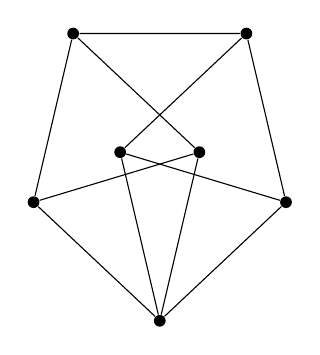
\begin{tikzpicture}[scale = 2.2]
        \node[circle, fill = black, inner sep = 1.5pt] (a) at (0, 0) {};
        \node[circle, fill = black, inner sep = 1.5pt] (p1) at (76.7787:1) {};
        \node[circle, fill = black, inner sep = 1.5pt] (q1) at (136.7787:1) {};
        \node[circle, fill = black, inner sep = 1.5pt] (t1) at (106.7787:1.7321) {};
        \node[circle, fill = black, inner sep = 1.5pt] (p2) at (43.2213:1) {};
        \node[circle, fill = black, inner sep = 1.5pt] (q2) at (103.2213:1) {};
        \node[circle, fill = black, inner sep = 1.5pt] (t2) at (73.2213:1.7321) {};
        \draw (a) -- (p1) -- (q1) -- (a);
        \draw (p1) -- (t1) -- (q1);
        \draw (a) -- (p2) -- (q2) -- (a);
        \draw (p2) -- (t2) -- (q2);
        \draw (t1) -- (t2);
    \end{tikzpicture}
\end{figure}
We thus conclude that $\chi(G) \geq 4$.

We can actually show that $\chi(G) \leq 7$. Indeed, consider the hexagonal tessellation of the plane. The point is that for a tessellation with hexagons of some diameter,
\begin{enumerate}
    \item all points in any given hexagon are of the same colour
    \item each hexagon and its $6$ neighbours have different colours
\end{enumerate}
Then, we can repeat colours \textit{after} a unit of $7$ (consisting of a hexagon and its neighbours).

% [FILLED] the diameter of the hexagons, and why the colouring is proper, supplied on 2026-10-07; the lecture gave neither
Take the hexagons to have diameter $d$ with $\frac{2}{\sqrt{21} - 2} < d < 1$---say $d = 0.9$---and give each boundary point to just one of the hexagons it lies on. Two points of one hexagon are less than $1$ apart, so giving a hexagon a single colour breaks nothing. The centres of neighbouring hexagons are $\frac{\sqrt{3}}{2} d$ apart, and in the colouring below the nearest hexagon of the same colour as a given one is two steps away in one direction and one in the next, so two same-coloured centres are at distance at least $\sqrt{7} \cdot \frac{\sqrt{3}}{2} d = \frac{\sqrt{21}}{2} d$. Every point of a hexagon is within $\frac{d}{2}$ of its centre, so two points of the same colour in different hexagons are at distance at least $\frac{\sqrt{21}}{2} d - d > 1$. No two points at distance exactly $1$ share a colour, and $\chi(G) \leq 7$.
\begin{figure}[H]
    \centering
    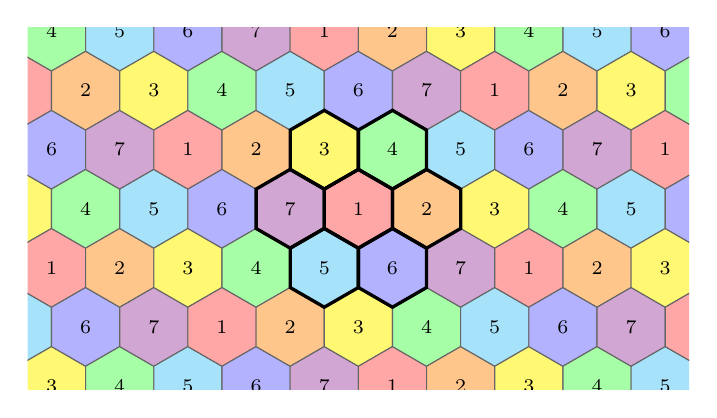
\begin{tikzpicture}
        \def\hexfills{{"red!35", "orange!45", "yellow!55", "green!35", "cyan!35", "blue!30", "violet!35"}}
        \clip (-4.2, -2.3) rectangle (4.2, 2.3);
        \foreach \hq in {-8, ..., 8}{
            \foreach \hr in {-4, ..., 4}{
                \pgfmathsetmacro{\x}{0.866 * (\hq + 0.5 * \hr)}
                \pgfmathsetmacro{\y}{0.75 * \hr}
                \pgfmathtruncatemacro{\hexc}{mod(mod(\hq + 3 * \hr, 7) + 7, 7)}
                \pgfmathtruncatemacro{\hexnum}{\hexc + 1}
                \pgfmathparse{\hexfills[\hexc]}
                \edef\hexfill{\pgfmathresult}
                \filldraw[fill = \hexfill, draw = black!60, shift = {(\x, \y)}] (30:0.5) -- (90:0.5) -- (150:0.5) -- (210:0.5) -- (270:0.5) -- (330:0.5) -- cycle;
                \node[font = \scriptsize] at (\x, \y) {$\hexnum$};
            }
        }
        \foreach \hq/\hr in {0/0, 1/0, -1/0, 0/1, 0/-1, 1/-1, -1/1}{
            \pgfmathsetmacro{\x}{0.866 * (\hq + 0.5 * \hr)}
            \pgfmathsetmacro{\y}{0.75 * \hr}
            \draw[very thick, shift = {(\x, \y)}] (30:0.5) -- (90:0.5) -- (150:0.5) -- (210:0.5) -- (270:0.5) -- (330:0.5) -- cycle;
        }
    \end{tikzpicture}
\end{figure}

\subsection{Compactness}

Now for a topological detour!

Recall that a space is compact iff the closed sets satisfy the finite intersection property: for closed sets $Y_{\alpha}$, with $\alpha \in I$, if $\bigcap_{\alpha \in J} Y_{\alpha}$ is nonempty for all finite $J \ssq I$, then $\bigcap_{\alpha \in I} Y_{\alpha}$ is nonempty as well.

We'll use this property (and Tychonoff) to prove a `compactness theorem' for the chromatic number of the plane.

\begin{boxtheorem} \label{Ch2:Thm:Compactness_Chromatic}
    For any graph $G$,
    \begin{align*}
        \chi(G) = \sup\setst{\chi(H)}{H \ssq G \text{ and } H \text{ is finite}}
    \end{align*}
\end{boxtheorem}

First, a lemma.

\begin{boxlemma} \label{Ch2:Lemma:Compactness}
    If every finite subgraph $B$ of $G$ is $k$-colourable, then so is $G$.
\end{boxlemma}
\begin{proof}
    Consider $[k]$ with the discrete topology and $[k]^{V(G)}$ with the product topology. Note that $[k]^{V(G)}$ is the set of all (not necessarily proper) colourings of $G$.

    For all $e \in E(G)$, define
    \begin{align*}
        P_e = \setst{c \in [k]^{V(G)}}{c(u) \ne c(v) \text{ for } e = \set{u, v}}
    \end{align*}
    It is possible to show that $P_e$ is clopen in $[k]^{V(G)}$: it is the preimage of the clopen set $\setst{(a, b) \in [k]^2}{a \neq b}$ under the projection onto the coordinates $u$ and $v$, which is continuous. % [FILLED] the reason after the colon was supplied on 2026-10-07

    % [FILLED] from ``the edges in $J$'' to the end of the proof, supplied on 2026-10-07: the lecture stopped at the display
    If every finite subgraph can be $k$-coloured, then for all finite $J \ssq E(G)$, $\bigcap_{e \in J} P_{e} \ne \emptyset$: the edges in $J$ span a finite subgraph, a proper $k$-colouring of it extends to all of $V(G)$ by colouring the remaining vertices arbitrarily, and the result lies in every $P_e$ with $e \in J$. By Tychonoff's theorem $[k]^{V(G)}$ is compact, the $P_e$ are closed, and so the finite intersection property gives $\bigcap_{e \in E(G)} P_e \ne \emptyset$. Any $c$ in that intersection has $c(u) \ne c(v)$ for every edge $\set{u, v}$, ie, is a proper $k$-colouring of $G$.
\end{proof}

% [FILLED] the deduction of the theorem from the lemma, supplied on 2026-10-07; the lecture stated the theorem, said ``first, a lemma'', and never came back
\begin{proof}[Proof of \Cref{Ch2:Thm:Compactness_Chromatic}]
    Every subgraph $H$ of $G$ has $\chi(H) \leq \chi(G)$, so the supremum is at most $\chi(G)$. Conversely, if the supremum is some finite $k$, then every finite subgraph is $k$-colourable, so $G$ is by \Cref{Ch2:Lemma:Compactness}, and $\chi(G) \leq k$.
\end{proof}

